\documentclass[11pt]{article}

% Paquetes y configuraciones adicionales
\usepackage{graphicx}
\usepackage[export]{adjustbox}
\usepackage{caption}
\usepackage{float}
\usepackage{titlesec}
\usepackage{geometry}
\usepackage[hidelinks]{hyperref}
\usepackage{titling}
\usepackage{titlesec}
\usepackage{parskip}
\usepackage{wasysym}
\usepackage{tikzsymbols}
\usepackage{fancyvrb}
\usepackage{xurl}
\usepackage{hyperref}
\usepackage{subcaption}

\usepackage{listings}
\usepackage{xcolor}

\usepackage[spanish]{babel}

\newcommand{\subtitle}[1]{
  \posttitle{
    \par\end{center}
    \begin{center}\large#1\end{center}
    \vskip0.5em}
}

% Configura los márgenes
\geometry{
  left=2cm,   % Ajusta este valor al margen izquierdo deseado
  right=2cm,  % Ajusta este valor al margen derecho deseado
  top=3cm,
  bottom=3cm,
}

% Configuración de los títulos de las secciones
\titlespacing{\section}{0pt}{\parskip}{\parskip}
\titlespacing{\subsection}{0pt}{\parskip}{\parskip}
\titlespacing{\subsubsection}{0pt}{\parskip}{\parskip}

% Redefinir el formato de los capítulos y añadir un punto después del número
\makeatletter
\renewcommand{\@makechapterhead}[1]{%
  \vspace*{0\p@} % Ajusta este valor para el espaciado deseado antes del título del capítulo
  {\parindent \z@ \raggedright \normalfont
    \ifnum \c@secnumdepth >\m@ne
        \huge\bfseries \thechapter.\ % Añade un punto después del número
    \fi
    \interlinepenalty\@M
    #1\par\nobreak
    \vspace{10pt} % Ajusta este valor para el espacio deseado después del título del capítulo
  }}
\makeatother

% Configura para que cada \chapter no comience en una pagina nueva
\makeatletter
\renewcommand\chapter{\@startsection{chapter}{0}{\z@}%
    {-3.5ex \@plus -1ex \@minus -.2ex}%
    {2.3ex \@plus.2ex}%
    {\normalfont\Large\bfseries}}
\makeatother

% Configurar los colores para el código
\definecolor{codegreen}{rgb}{0,0.6,0}
\definecolor{codegray}{rgb}{0.5,0.5,0.5}
\definecolor{codepurple}{rgb}{0.58,0,0.82}
\definecolor{backcolour}{rgb}{0.95,0.95,0.92}

% Configurar el estilo para el código
\lstdefinestyle{mystyle}{
  backgroundcolor=\color{backcolour},   
  commentstyle=\color{codegreen},
  keywordstyle=\color{magenta},
  numberstyle=\tiny\color{codegray},
  stringstyle=\color{codepurple},
  basicstyle=\ttfamily\footnotesize,
  breakatwhitespace=false,         
  breaklines=true,                 
  captionpos=b,                    
  keepspaces=true,                 
  numbers=left,                    
  numbersep=5pt,                  
  showspaces=false,                
  showstringspaces=false,
  showtabs=false,                  
  tabsize=2
}

\begin{document}

\title{Práctica 1: Análisis de Algoritmos}
\author{Adrián Grassin Luis}
\date{\today}

\maketitle

\section{Principios SOLID}
Los principios SOLID son guías fundamentales para el diseño orientado a objetos que mejoran la mantenibilidad y escalabilidad del software. El principio de responsabilidad única (SRP) establece que una clase debe tener una única razón para cambiar, es decir, debe encapsular una única funcionalidad o responsabilidad del sistema.

\section{Patrón Estrategia}
El patrón estrategia permite definir una familia de algoritmos intercambiables en tiempo de ejecución. Cada algoritmo se encapsula en una clase separada que implementa una interfaz común, permitiendo que los algoritmos varíen independientemente de los clientes que los utilizan. En esta práctica, se aplica este patrón para implementar diferentes estrategias de multiplicación de matrices.

\section{Análisis de Algoritmos}

\subsection{Arquitectura de Ejecución}
\begin{itemize}
    \item \textbf{CPU:} AMD Ryzen 5600X (6 cores, 12 threads)
    \item \textbf{GPU:} AMD Radeon RX 7800 XT (16GB VRAM)
    \item \textbf{RAM:} 32GB DDR4
    \item \textbf{Framework:} .NET 8.0
\end{itemize}

\subsection{Resultados Experimentales}
\begin{figure}[h]
    \centering
    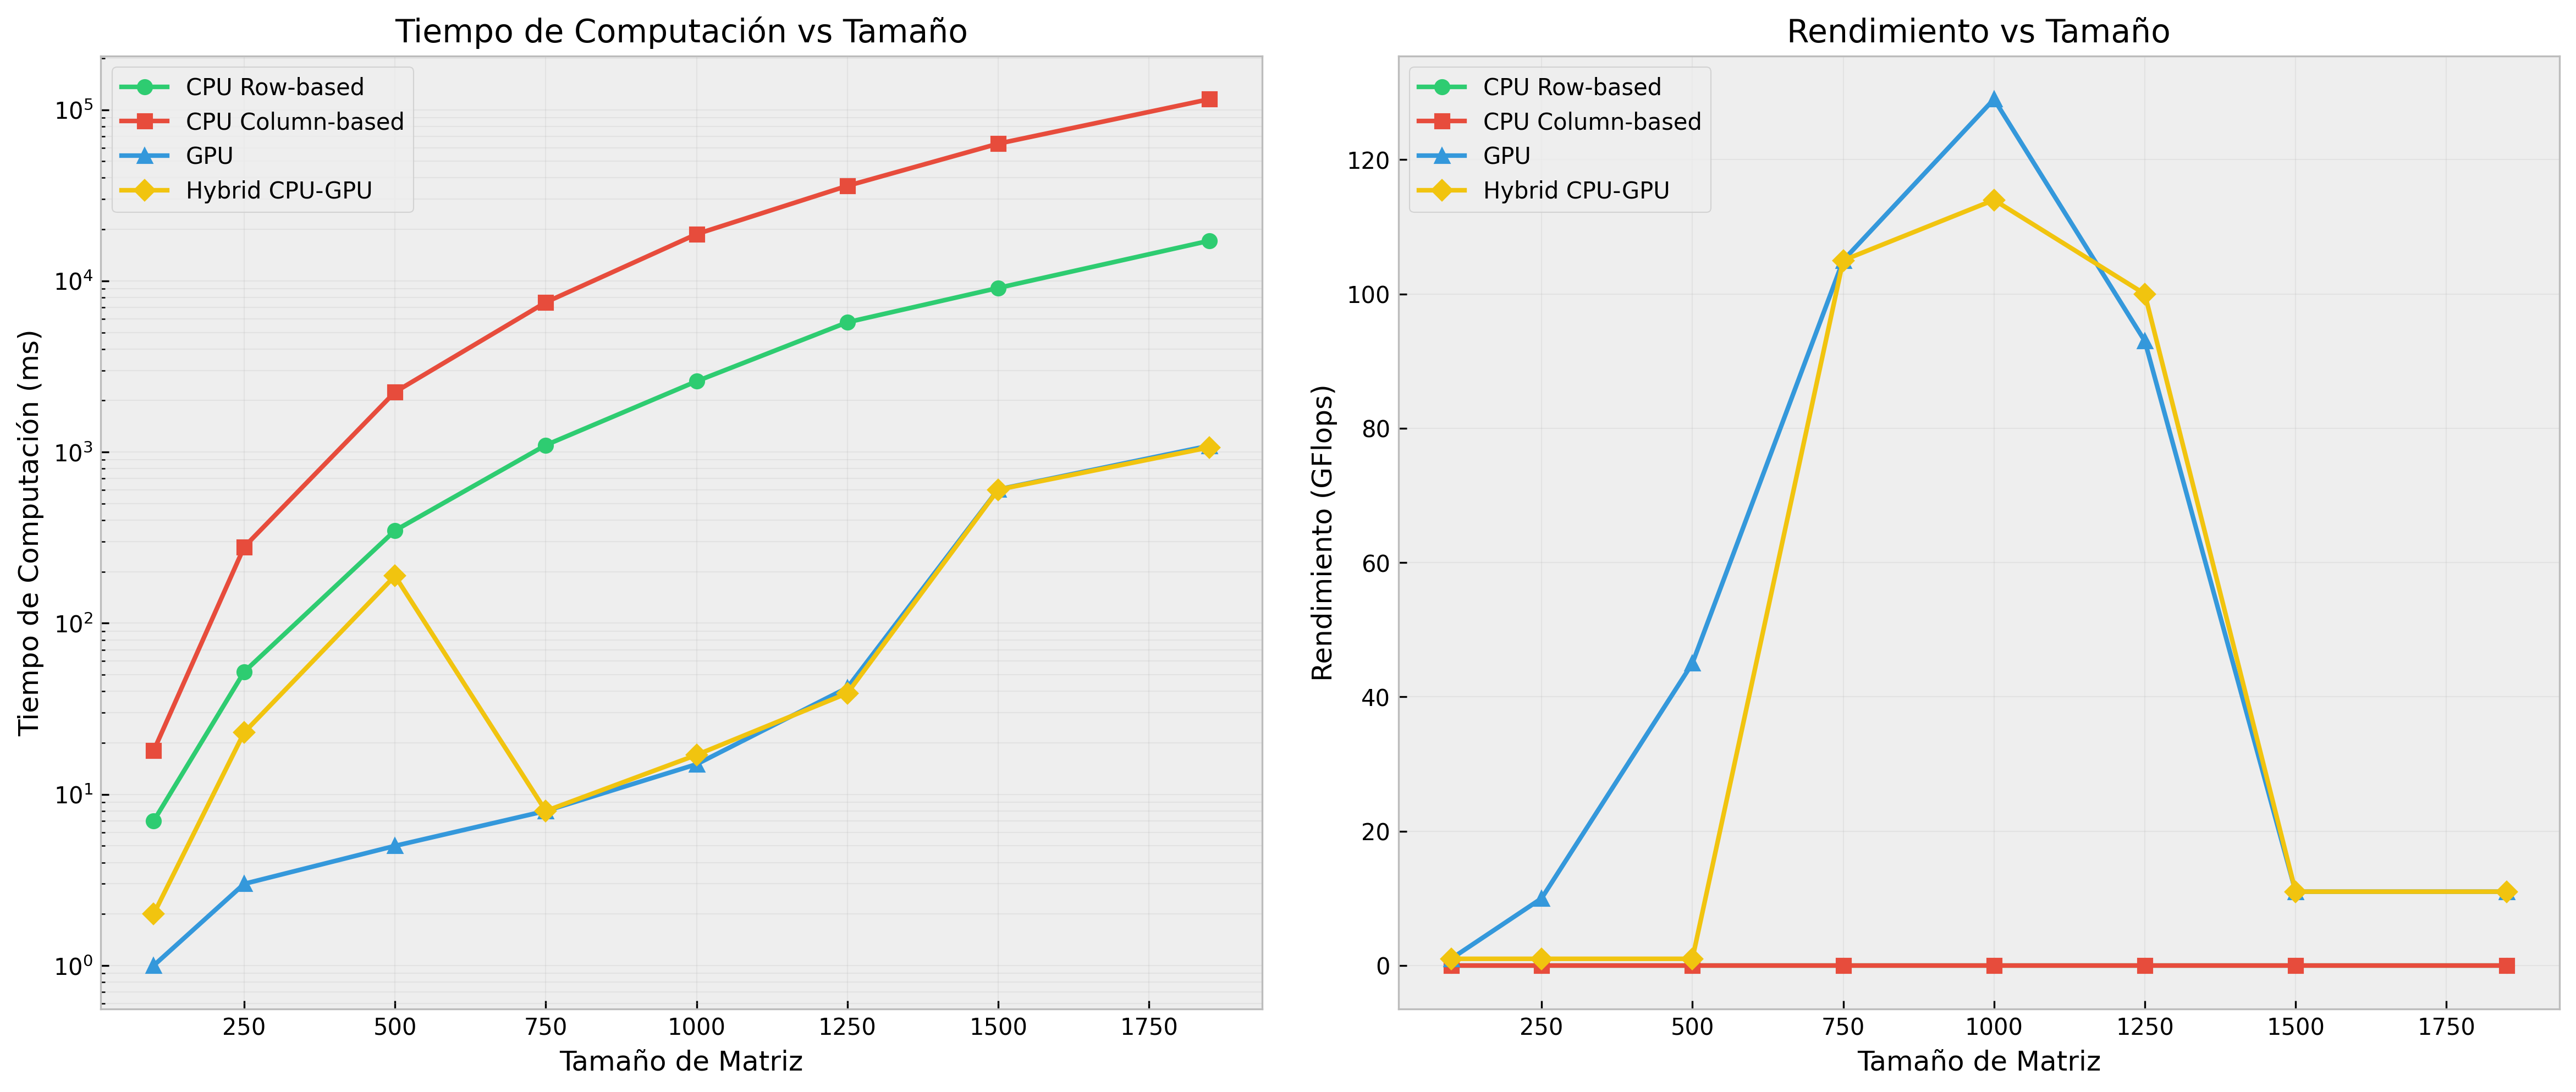
\includegraphics[width=\textwidth]{grafica.png}
    \caption{Comparación de rendimiento: Tiempo de computación (izq.) y GFlops (der.)}
    \label{fig:performance}
\end{figure}

\subsection{Análisis y Conclusiones}
Los resultados muestran tres comportamientos distintivos según el tamaño de las matrices:

\begin{itemize}
    \item \textbf{Matrices pequeñas < (500x500):} La implementación por filas es superior debido a la mejor localidad de memoria y menor overhead. La versión por columnas muestra un rendimiento significativamente peor debido a los fallos de caché.
    
    \item \textbf{Matrices medianas (500x500-1000x1000):} La GPU comienza a mostrar ventajas, alcanzando hasta 105 GFlops en matrices de 750x750, comparado con 0.77 GFlops de la CPU.
    
    \item \textbf{Matrices grandes > (1000x1000):} La diferencia entre implementaciones se amplifica. La versión por columnas muestra el peor rendimiento (0.11 GFlops), mientras que la GPU mantiene un rendimiento superior (11-129 GFlops).
\end{itemize}

La implementación por filas supera consistentemente a la versión por columnas debido a la arquitectura de memoria de la CPU, que favorece accesos secuenciales. La GPU muestra una clara ventaja en matrices grandes debido a su capacidad de procesamiento paralelo masivo.

\end{document}
